% !TeX program = xelatex
\documentclass[a4paper,10pt]{article}

% ============================================================================
% កញ្ចប់បណ្ណាល័យ (Packages) – តាមលំនាំ NGS Preah Krasang (ls_plan.tex)
% បរិបទ៖ គ្មានស្លាយ LCD និងគ្មានសម្ភារៈកាត់បិទស្មុគស្មាញ — ប្រើសន្លឹកកិច្ចការសិស្ស (ស-ខ្មៅ) ជាគោល
% ============================================================================
\usepackage[a4paper, left=0.95cm, right=0.95cm, top=0.85cm, bottom=0.92cm, footskip=0.52cm]{geometry}
\usepackage{amsmath}
\usepackage{unicode-math}
\usepackage{fontspec}
\usepackage{array, longtable, multirow, colortbl}
\usepackage[table]{xcolor}
\usepackage{enumitem}
\usepackage{pifont}
\usepackage{fancyhdr}
\usepackage{tikz}
\usetikzlibrary{calc, arrows.meta, angles, quotes, decorations.markings, decorations.pathreplacing, patterns, babel}

% LaTeX 2025 + longtable v4.24 compatibility guard
\makeatletter
\let\@expl@@@mark@update@singlecol@structures@@\relax
\makeatother

% ============================================================================
% ការកំណត់ពុម្ពអក្សរ (Fonts Configuration - Cross-Platform Windows + Cloud fonts/)
% ============================================================================
\providecommand{\NGSFindFonts}{%
  \IfFileExists{C:/Windows/Fonts/cambria.ttc}{%
    \def\NGSSysPath{C:/Windows/Fonts/}%
    \def\NGSUserPath{C:/Users/KIT/AppData/Local/Microsoft/Windows/Fonts/}%
  }{%
    \IfFileExists{./fonts/KhmerOSsiemreap.ttf}{\def\NGSSysPath{./fonts/}\def\NGSUserPath{./fonts/}}{%
    \IfFileExists{../fonts/KhmerOSsiemreap.ttf}{\def\NGSSysPath{../fonts/}\def\NGSUserPath{../fonts/}}{%
    \IfFileExists{../../fonts/KhmerOSsiemreap.ttf}{\def\NGSSysPath{../../fonts/}\def\NGSUserPath{../../fonts/}}{%
    \IfFileExists{../../../fonts/KhmerOSsiemreap.ttf}{\def\NGSSysPath{../../../fonts/}\def\NGSUserPath{../../../fonts/}}{%
    \IfFileExists{../../../../fonts/KhmerOSsiemreap.ttf}{\def\NGSSysPath{../../../../fonts/}\def\NGSUserPath{../../../../fonts/}}{%
    \IfFileExists{../../../../../fonts/KhmerOSsiemreap.ttf}{\def\NGSSysPath{../../../../../fonts/}\def\NGSUserPath{../../../../../fonts/}}{%
    \IfFileExists{../../../../../../fonts/KhmerOSsiemreap.ttf}{\def\NGSSysPath{../../../../../../fonts/}\def\NGSUserPath{../../../../../../fonts/}}{%
      \def\NGSSysPath{../../../../../../../fonts/}\def\NGSUserPath{../../../../../../../fonts/}%
    }}}}}}}%
  }%
}
\NGSFindFonts

\setmathfont[
  Path={\NGSSysPath},
  FontIndex=1,
  Scale=1.02
]{cambria.ttc}

\defaultfontfeatures{Ligatures=TeX}

\setmainfont[
  Path={\NGSUserPath},
  Extension=.ttf,
  Script=Khmer,
  BoldFont={KhmerOSsiemreap},
  BoldFeatures={FakeBold=1.8},
  ItalicFont={KhmerOSsiemreap},
  ItalicFeatures={FakeSlant=0.25},
  BoldItalicFont={KhmerOSsiemreap},
  BoldItalicFeatures={FakeBold=1.8, FakeSlant=0.25}
]{KhmerOSsiemreap}

\newfontfamily\muol[
  Path={\NGSUserPath},
  Extension=.ttf,
  Script=Khmer
]{KhmerOSmuollight}

\newfontfamily\TimesEn[
  Path={\NGSSysPath},
  Extension=.ttf,
  Scale=1.00,
  BoldFont={timesbd},
  ItalicFont={timesi},
  BoldItalicFont={timesbi}
]{times}

\newfontfamily\NagaBold[
  Path={\NGSUserPath},
  Extension=.ttf
]{AKbalthom Naga Bold}

\newfontfamily\CalibriFont[
  Path={\NGSSysPath},
  Extension=.ttf
]{calibri}

\newfontfamily\Tacteing[
  Path={\NGSUserPath}
]{TACTENG.TTF}

\newfontfamily\CourierBullet[
  Path={\NGSSysPath},
  Extension=.ttf
]{cour}
\newcommand{\wcirc}{{\CourierBullet\fontsize{9.5pt}{11pt}\selectfont o}}

% ក្បួនកាត់ពាក្យខ្មែរ (Khmer word wrapping)
\XeTeXlinebreaklocale "km"
\XeTeXlinebreakskip = 0pt plus 1pt minus 0.1pt

% ============================================================================
% ការកំណត់ពណ៌ និងទម្រង់ទំព័រ (Colors & Page Style)
% ============================================================================
\definecolor{stepgray}{HTML}{D9D9D9}
\definecolor{headgray}{HTML}{F2F2F2}
\definecolor{boxgray}{HTML}{D9D9D9}
\definecolor{darkred}{HTML}{C00000}
\definecolor{red5e}{HTML}{FF0000}

\pagestyle{fancy}
\fancyhf{}
\renewcommand{\headrulewidth}{0pt}
\fancyfoot[R]{\CalibriFont\fontsize{11pt}{13pt}\selectfont\thepage}

\setlength{\parindent}{0pt}
\setlength{\parskip}{0pt}
\setlength{\tabcolsep}{3.8pt}

\newcolumntype{L}[1]{>{\raggedright\arraybackslash}p{#1}}

% ============================================================================
% ម៉ាក្រូជំនួយ (Helper Macros)
% ============================================================================
\newcommand{\en}[1]{{\TimesEn #1}}
\newcommand{\enbf}[1]{{\TimesEn\textbf{#1}}}
\newcommand{\unit}[1]{\,\text{\en{#1}}}
\newcommand{\fiveE}[1]{{\NagaBold\fontsize{9.5pt}{13pt}\selectfont\textcolor{red5e}{#1}}}
\newcommand{\timenote}[1]{\textcolor{darkred}{\textit{#1}}}
\newcommand{\redsub}[1]{\textcolor{darkred}{#1}}
\newcommand{\graybox}[1]{\colorbox{boxgray}{\strut\hspace{2pt}#1\hspace{2pt}}}
\newcommand{\ditem}{\tikz[baseline=-0.5ex]\fill (0,0.42ex) -- (0.42ex,0) -- (0,-0.42ex) -- (-0.42ex,0) -- cycle;\hspace{0.3em}}
\newcommand{\cnum}[1]{{\fontsize{10.5pt}{12pt}\selectfont\ding{\numexpr181+#1\relax}}\hspace{0.15em}}
\newcommand{\cfig}[1]{\par\vspace{3pt}{\centering #1\par}\vspace{3pt}}
\newcommand{\stepheader}[1]{\multicolumn{3}{|c|}{\cellcolor{stepgray}\muol #1} \\* \noalign{\hrule height 0.4pt}}
\newcommand{\fboxb}[1]{\begingroup\setlength{\fboxsep}{1.5pt}\fbox{#1}\endgroup}

% ក្បាច់ក្រោមបាវចនា (Tacteing Font - Keyboard '3')
\newcommand{\khmflourish}{{\Tacteing\fontsize{36pt}{14pt}\selectfont\raisebox{-5pt}{3}}}

% ============================================================================
% ម៉ាក្រូគូសរូប TikZ ស-ខ្មៅ ១០០% សម្រាប់គូសលើក្ដារខៀន និងសន្លឹកកិច្ចការសិស្ស
% ============================================================================

% ១. ជំហានទី២ E1 Engage: បញ្ហាបត់ក្រដាស ៦ ដង និងប្រអប់ចាក់សោ (-2)^6 vs -2^6
\newcommand{\figEngageEXP}{%
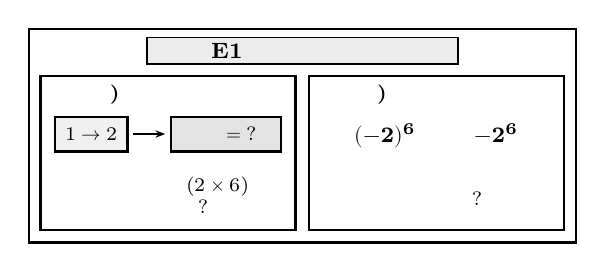
\begin{tikzpicture}[scale=0.92, every node/.style={font=\scriptsize, text=black}]
  \draw[black, line width=0.95pt] (0,0) rectangle (7.55,2.95);
  \node[fill=gray!15, draw=black, line width=0.6pt, inner sep=2pt, font=\footnotesize\bfseries] at (3.775,2.65) {បេសកកម្ម \en{E1}៖ បត់ក្រដាស ៦ ដង និងល្បែងសញ្ញាដក};

  % ឆ្វេង៖ បត់ក្រដាស
  \draw[black, line width=0.8pt] (0.16,0.18) rectangle (3.68,2.30);
  \node[font=\scriptsize\bfseries] at (1.92,2.04) {១) បត់ពាក់កណ្ដាល ៦ ដង};
  \draw[black, line width=0.8pt, fill=gray!12] (0.36,1.26) rectangle (1.36,1.74);
  \node at (0.86,1.50) {$1\to 2$};
  \draw[black, line width=0.8pt, -{Stealth[length=3.5pt]}] (1.44,1.50) -- (1.88,1.50);
  \draw[black, line width=0.8pt, fill=gray!22] (1.96,1.26) rectangle (3.48,1.74);
  \node at (2.72,1.50) {៦ ដង $= ?$};
  \node[align=center] at (1.92,0.66) {តើបាន \textbf{១២ ស្រទាប់} ($2\times 6$)\\ឬ \textbf{៦៤ ស្រទាប់}?};

  % ស្ដាំ៖ (-2)^6 vs -2^6
  \draw[black, line width=0.8pt] (3.86,0.18) rectangle (7.39,2.30);
  \node[font=\scriptsize\bfseries] at (5.625,2.04) {២) វង់ក្រចក និងសញ្ញាដក};
  \node[font=\footnotesize] at (5.625,1.48) {$\mathbf{(-2)^6}$ \;\;ធៀប\;\; $\mathbf{-2^6}$};
  \node[align=center] at (5.625,0.66) {តើលទ្ធផល\textbf{ស្មើគ្នា}\\ឬ\textbf{ផ្ទុយសញ្ញាគ្នា}?};
\end{tikzpicture}}

% ២. E2 Act 1: តារាងកំណើនទ្វេដង 2^n ធៀបនឹងផលគុណ 2n លើសន្លឹកកិច្ចការ
\newcommand{\figDoublingEXP}{%
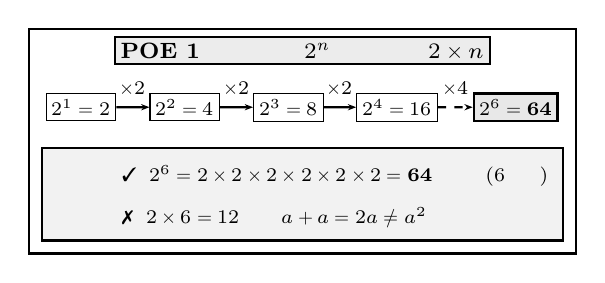
\begin{tikzpicture}[scale=0.92, every node/.style={font=\scriptsize, text=black}]
  \draw[black, line width=0.95pt] (0,0) rectangle (7.55,3.10);
  \node[fill=gray!15, draw=black, line width=0.6pt, inner sep=2pt, font=\footnotesize\bfseries] at (3.775,2.80) {\en{POE 1}៖ កំណើនស្វ័យគុណ $2^n$ ធៀបនឹងអន្ទាក់ $2\times n$};

  \node[draw=black, fill=white, inner sep=2pt] (F1) at (0.72,2.02) {$2^1=2$};
  \node[draw=black, fill=white, inner sep=2pt] (F2) at (2.15,2.02) {$2^2=4$};
  \node[draw=black, fill=white, inner sep=2pt] (F3) at (3.58,2.02) {$2^3=8$};
  \node[draw=black, fill=white, inner sep=2pt] (F4) at (5.08,2.02) {$2^4=16$};
  \node[draw=black, fill=gray!18, line width=0.95pt, inner sep=2pt] (F6) at (6.72,2.02) {$2^6=\mathbf{64}$};

  \draw[black, line width=0.8pt, -{Stealth[length=3pt]}] (F1) -- node[above=1pt]{$\times 2$} (F2);
  \draw[black, line width=0.8pt, -{Stealth[length=3pt]}] (F2) -- node[above=1pt]{$\times 2$} (F3);
  \draw[black, line width=0.8pt, -{Stealth[length=3pt]}] (F3) -- node[above=1pt]{$\times 2$} (F4);
  \draw[black, line width=0.8pt, dashed, -{Stealth[length=3pt]}] (F4) -- node[above=1pt]{$\times 4$} (F6);

  \draw[black, line width=0.8pt, fill=gray!10] (0.18,0.18) rectangle (7.37,1.46);
  \node[anchor=west] at (0.30,1.08) {\textbf{ផ្លូវត្រូវ} \ding{51}៖ $2^6 = 2\times 2\times 2\times 2\times 2\times 2 = \mathbf{64}$ ស្រទាប់ ($6$ កត្តា)};
  \node[anchor=west] at (0.30,0.50) {\textbf{អន្ទាក់ខុស} \ding{55}៖ $2\times 6 = 12$ \;និង\; $a+a=2a \neq a^2$};
\end{tikzpicture}}

% ៣. E2 Act 2: ប្រអប់ចាក់សោ Lock-Box (-2)^6 vs -2^6 និងធ្នូផ្គូផ្គងសញ្ញា
\newcommand{\figLockBoxEXP}{%
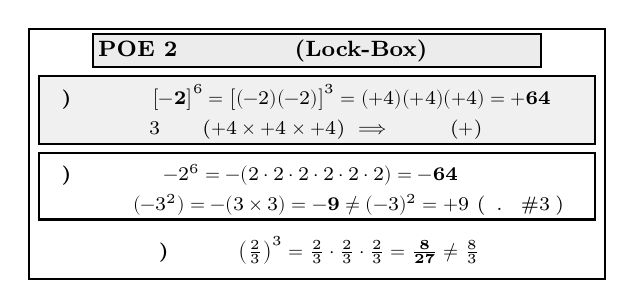
\begin{tikzpicture}[scale=0.92, every node/.style={font=\scriptsize, text=black}]
  \draw[black, line width=0.95pt] (0,0) rectangle (7.95,3.45);
  \node[fill=gray!15, draw=black, line width=0.6pt, inner sep=2pt, font=\footnotesize\bfseries] at (3.975,3.15) {\en{POE 2}៖ ប្រអប់ចាក់សោគោល \en{(Lock-Box)} និងផ្គូផ្គងសញ្ញា};

  % ជួរលើ៖ (-2)^6 = +64
  \draw[black, line width=0.9pt, fill=gray!12] (0.14,1.86) rectangle (7.81,2.80);
  \node[anchor=west] at (0.24,2.50) {\textbf{១) មានវង់ក្រចក៖} $\big[\mathbf{-2}\big]^6 = \big[(-2)(-2)\big]^3 = (+4)(+4)(+4) = \mathbf{+64}$};
  \node[anchor=west] at (0.45,2.06) {ផ្គូផ្គងដកបាន $3$ គូពេញ ($+4\times +4\times +4$) $\implies$ សញ្ញាបូក ($+$)};

  % ជួរក្រោម៖ -2^6 = -64 និង (-3^2) = -9
  \draw[black, line width=0.85pt] (0.14,0.82) rectangle (7.81,1.74);
  \node[anchor=west] at (0.24,1.44) {\textbf{២) គ្មានវង់ក្រចក៖} $-2^6 = -(2\cdot 2\cdot 2\cdot 2\cdot 2\cdot 2) = \mathbf{-64}$};
  \node[anchor=west] at (0.45,1.02) {ដូចគ្នានឹង $(-3^2) = -(3\times 3) = \mathbf{-9} \neq (-3)^2 = +9$ (ទំ.២៥ \#3ក)};

  \node at (3.975,0.40) {\textbf{៣) គោលប្រភាគ៖} $\left(\frac{2}{3}\right)^3 = \frac{2}{3}\cdot\frac{2}{3}\cdot\frac{2}{3} = \mathbf{\frac{8}{27}} \neq \frac{8}{3}$};
\end{tikzpicture}}

% ៤. E3 Explain: ដ្យាក្រាម Hub-and-Spoke a^n + បណ្ដុំអាទិភាពប្រមាណវិធី ៣ ថ្នាក់
\newcommand{\figExplainHubEXP}{%
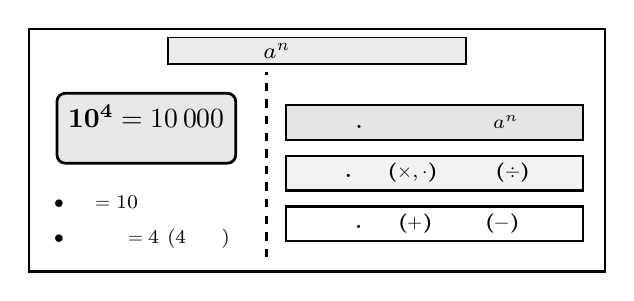
\begin{tikzpicture}[scale=0.92, every node/.style={font=\scriptsize, text=black}]
  \draw[black, line width=0.95pt] (0,0) rectangle (7.95,3.35);
  \node[fill=gray!15, draw=black, line width=0.6pt, inner sep=2pt, font=\footnotesize\bfseries] at (3.975,3.05) {ស្នូលស្វ័យគុណ $a^n$ និងថ្នាក់អាទិភាពប្រមាណវិធី};

  % ឆ្វេង៖ សមាសភាគ 3 ផ្នែកនៃ a^n
  \node[draw=black, line width=1.0pt, fill=gray!18, rounded corners=3pt, inner sep=4pt, align=center] at (1.62,1.98) {\normalsize $\mathbf{10^4} = 10\,000$\\[1pt]ហៅថា \textbf{ស្វ័យគុណ}};
  \node[anchor=west] at (0.22,0.96) {$\bullet$ គោល $= 10$};
  \node[anchor=west] at (0.22,0.46) {$\bullet$ និទស្សន្ត $= 4$ ($4$ កត្តា)};

  \draw[black, line width=0.8pt, dashed] (3.28,0.20) -- (3.28,2.75);

  % ស្ដាំ៖ បណ្ដុំអាទិភាព ៣ ថ្នាក់ច្បាស់ៗ
  \node[font=\scriptsize\bfseries] at (5.60,2.56) {លំដាប់អាទិភាពគណនា};
  \draw[black, line width=0.9pt, fill=gray!20] (3.55,1.82) rectangle (7.65,2.30);
  \node at (5.60,2.06) {\textbf{១. វង់ក្រចក និងស្វ័យគុណ $a^n$}};
  \draw[black, line width=0.85pt, fill=gray!10] (3.55,1.12) rectangle (7.65,1.60);
  \node at (5.60,1.36) {\textbf{២. គុណ ($\times,\cdot$) និង ចែក ($\div$)}};
  \draw[black, line width=0.8pt, fill=white] (3.55,0.42) rectangle (7.65,0.90);
  \node at (5.60,0.66) {\textbf{៣. បូក ($+$) និង ដក ($-$)}};
\end{tikzpicture}}

% ៥. E5 Diagnostic Cards A-D លើសន្លឹកកិច្ចការសិស្ស
\newcommand{\figExitCardsEXP}{%
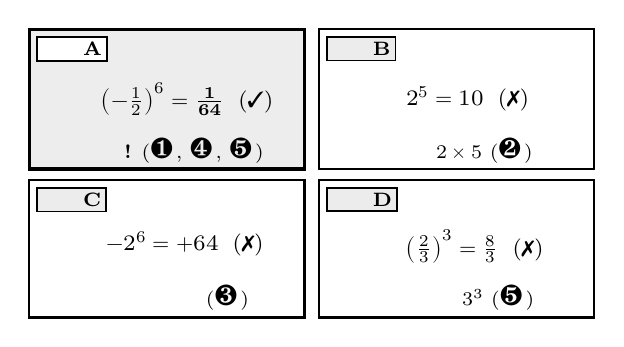
\begin{tikzpicture}[scale=0.92, every node/.style={font=\scriptsize, text=black}]
  % កាត A (CHECK)
  \draw[black, line width=1.1pt, fill=gray!14] (0,2.05) rectangle (3.80,3.98);
  \node[anchor=north west, fill=white, draw=black, line width=0.6pt, inner sep=1.8pt] at (0.10,3.88) {\textbf{ជម្រើស \en{A}}};
  \node[font=\footnotesize] at (2.18,3.02) {$\left(-\frac{1}{2}\right)^6 = \mathbf{\frac{1}{64}}$ \;(\ding{51})};
  \node at (1.90,2.30) {\textbf{ត្រឹមត្រូវ!} (\cnum{1}, \cnum{4}, \cnum{5})};

  % កាត B (X)
  \draw[black, line width=0.9pt] (4.00,2.05) rectangle (7.80,3.98);
  \node[anchor=north west, fill=gray!15, draw=black, line width=0.6pt, inner sep=1.8pt] at (4.10,3.88) {\textbf{ជម្រើស \en{B}}};
  \node[font=\footnotesize] at (6.05,3.02) {$2^5 = 10$ \;(\ding{55})};
  \node at (5.90,2.30) {អន្ទាក់យក $2\times 5$ (\cnum{2})};

  % កាត C (X)
  \draw[black, line width=0.9pt] (0,0) rectangle (3.80,1.90);
  \node[anchor=north west, fill=gray!15, draw=black, line width=0.6pt, inner sep=1.8pt] at (0.10,1.80) {\textbf{ជម្រើស \en{C}}};
  \node[font=\footnotesize] at (2.15,1.02) {$-2^6 = +64$ \;(\ding{55})};
  \node at (1.90,0.28) {គ្មានវង់ក្រចកចាក់សោដក (\cnum{3})};

  % កាត D (X)
  \draw[black, line width=0.9pt] (4.00,0) rectangle (7.80,1.90);
  \node[anchor=north west, fill=gray!15, draw=black, line width=0.6pt, inner sep=1.8pt] at (4.10,1.80) {\textbf{ជម្រើស \en{D}}};
  \node[font=\footnotesize] at (6.15,0.98) {$\left(\frac{2}{3}\right)^3 = \frac{8}{3}$ \;(\ding{55})};
  \node at (5.90,0.28) {ភ្លេចលើកភាគបែង $3^3$ (\cnum{5})};
\end{tikzpicture}}

% 6. E4 Worked-Example Contrast Card (7.55cm x 3.25cm)
\newcommand{\figElaborateContrastEXP}{%
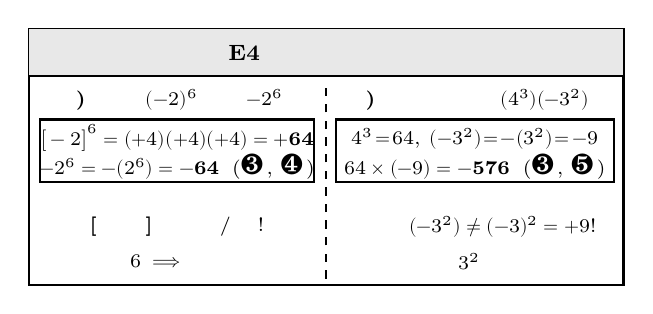
\begin{tikzpicture}[x=1cm, y=1cm, font=\scriptsize]
  \draw[black, line width=0.9pt] (0,0) rectangle (7.55,3.25);
  \fill[gray!18] (0,2.65) rectangle (7.55,3.25);
  \draw[black, line width=0.7pt] (0,2.65) -- (7.55,2.65);
  \node[font=\footnotesize\bfseries] at (3.775,2.95) {កាតស៊ើបអង្កេត \en{E4}៖ អាទិភាពប្រមាណវិធី និងប្រអប់ចាក់សោសញ្ញា};
  \draw[black, dashed, line width=0.6pt] (3.775,0.08) -- (3.775,2.58);
  % Left: (-2)^6 vs -2^6
  \node[font=\scriptsize\bfseries] at (1.88,2.35) {១) ប្រៀបធៀប $(-2)^6$ ទល់នឹង $-2^6$};
  \draw[black, line width=0.75pt] (0.14,1.30) rectangle (3.62,2.10);
  \node at (1.88,1.86) {$\big[-2\big]^6 = (+4)(+4)(+4) = \mathbf{+64}$};
  \node at (1.88,1.50) {$-2^6 = -(2^6) = \mathbf{-64}$ \;(\cnum{3}, \cnum{4})};
  \node at (1.88,0.74) {\textbf{[ចង្អុលអូស]} វង់ក្រចកមាន/គ្មាន!};
  \node at (1.88,0.30) {និទស្សន្តគូ $6 \implies$ សញ្ញាផ្ទុយគ្នាដាច់};
  % Right: (4^3)(-3^2)
  \node[font=\scriptsize\bfseries] at (5.66,2.35) {២) អន្ទាក់ក្នុងវង់ក្រចក $(4^3)(-3^2)$};
  \draw[black, line width=0.75pt] (3.90,1.30) rectangle (7.43,2.10);
  \node at (5.665,1.86) {$4^3\!=\!64,\; (-3^2)\!=\!-(3^2)\!=\!-9$};
  \node at (5.665,1.50) {$64\times(-9) = \mathbf{-576}$ \;(\cnum{3}, \cnum{5})};
  \node at (5.66,0.74) {ប្រយ័ត្ន៖ $(-3^2) \neq (-3)^2 = +9$!};
  \node at (5.66,0.30) {ធ្វើស្វ័យគុណ $3^2$ មុនដាក់សញ្ញាដក};
\end{tikzpicture}}

% ============================================================================
% ចាប់ផ្ដើមឯកសារ (Document Body — ពេញទំព័រ >=90%)
% ============================================================================
\begin{document}
\fontsize{10pt}{15.2pt}\selectfont

% -------------------- ក្បាលកិច្ចតែងការ (Header) --------------------
\begin{center}
  {\muol\fontsize{11pt}{16pt}\selectfont ព្រះរាជាណាចក្រកម្ពុជា}\\[2pt]
  {\muol\fontsize{10pt}{15pt}\selectfont ជាតិ សាសនា ព្រះមហាក្សត្រ}\\[1pt]
  \khmflourish
\end{center}

\vspace{-24pt}
{\muol\fontsize{9.5pt}{12.5pt}\selectfont
មន្ទីរអប់រំ យុវជន និងកីឡា ខេត្តកំពង់ធំ\\
ការិយាល័យអប់រំ យុវជន និងកីឡា ស្រុកកំពង់ស្វាយ\\
អនុវិទ្យាល័យព្រះក្រសាំង}

\vspace{1pt}
\begin{center}
  {\muol\fontsize{10pt}{14pt}\selectfont កិច្ចតែងការបង្រៀន}
\end{center}
\vspace{0pt}

% -------------------- ព័ត៌មានទូទៅ (Metadata) --------------------
{\renewcommand{\arraystretch}{0.98}
\hspace*{3.1cm}%
\begin{tabular}{@{}l l L{11.0cm}@{}}
  - \hspace{0.35cm} មុខវិជ្ជា & : & គណិតវិទ្យា ថ្នាក់ទី៨ (ពីជគណិត) \\
  - \hspace{0.35cm} ចំណងជើងមេរៀន & : & មេរៀនទី២៖ ស្វ័យគុណ \\
  - \hspace{0.35cm} ចំណងជើងរង & : & ២.១. សញ្ញាណស្វ័យគុណ (សៀវភៅពុម្ព ទំ.១៣–១៤ និងលំហាត់ ទំ.២៥) \\
  - \hspace{0.35cm} រយៈពេល & : & ១ ម៉ោងសិក្សា (៥០ នាទី) \\
  - \hspace{0.35cm} បង្រៀនដោយ & : & ហុក ប៊ុនថែន \\
  - \hspace{0.35cm} កាលបរិច្ឆេទ & : & ថ្ងៃចន្ទ ទី១៦ ខែវិច្ឆិកា ឆ្នាំ២០២៦ \\
\end{tabular}

\vspace{2pt}

% -------------------- I. វត្ថុបំណង (MoEYS 3 Domains) --------------------
\textbf{I.} {\muol វត្ថុបំណង}\\[1pt]
\hspace*{0.55cm}%
\begin{tabular}{@{}l l L{14.2cm}@{}}
  \wcirc \hspace{0.25cm} វិជ្ជាសម្បទា & : & សិស្សប្រាប់និយមន័យស្វ័យគុណ $\underbrace{a\times a\times\dots\times a}_{n\text{ កត្តា}} = a^n$ ($a\in\mathbb{Q},\; n\in\mathbb{Z}^+$), កំណត់គោល និទស្សន្ត និងរបៀបអានស្វ័យគុណ (ការេ គូប) ព្រមទាំងបែងចែកច្បាស់រវាង $(-a)^n$ និង $-a^n$ ។ \\
  \wcirc \hspace{0.25cm} បំណិនសម្បទា & : & សិស្សបំពេញសន្លឹកកិច្ចការស៊ើបអង្កេត សរសេរផលគុណកត្តាដូចគ្នាជាស្វ័យគុណ និងគណនាតម្លៃនៃស្វ័យគុណមានគោលជាចំនួនគត់ ប្រភាគ និងចំនួនអវិជ្ជមាន (ទំ.១៤ និង ទំ.២៥) បានត្រឹមត្រូវ ។ \\
  \wcirc \hspace{0.25cm} ចរិយាសម្បទា & : & សិស្សមានទម្លាប់ពិនិត្យវង់ក្រចក និងសញ្ញាដោយប្រុងប្រយ័ត្ន ចៀសវាងអន្ទាក់យកគោលគុណនិទស្សន្ត ($a^n\neq a\cdot n$) និងសហការផ្ទៀងផ្ទាត់ចម្លើយជាដៃគូលើសន្លឹកកិច្ចការយ៉ាងសកម្ម ។ \\
\end{tabular}

\vspace{2pt}

% -------------------- II. សម្ភារៈឧបទេស (No LCD, Worksheet-Centered) --------------------
\textbf{II.} {\muol សម្ភារៈឧបទេស}\\[1pt]
\hspace*{0.55cm}$\bullet$ \hspace{0.35cm} សៀវភៅសិក្សាគោលគណិតវិទ្យាថ្នាក់ទី៨ (ទំ.១៣–១៤, ២៥) ក្ដារខៀន ដីស សន្លឹកកិច្ចការសិស្ស ស-ខ្មៅ (\en{Worksheet\_EXP1} ទំព័រ ១–២ សម្រាប់បំពេញផ្ទាល់ដោយមិនប្រើស្លាយ \en{LCD} ឬសម្ភារៈកាត់បិទ) និងក្រដាសព្រាងបត់ផ្ទៀងផ្ទាត់

\vspace{2pt}

% -------------------- III. វិធីសាស្រ្តបង្រៀន --------------------
\textbf{III.} {\muol វិធីសាស្រ្តបង្រៀន}\\[1pt]
\hspace*{0.45cm}%
\begin{tabular}{@{}l l L{14.85cm}@{}}
  $\bullet$ \hspace{0.25cm} គោលវិធី & : & សិស្សមជ្ឈមណ្ឌល (បង្រៀនតាមសន្លឹកកិច្ចការស៊ើបអង្កេត និងក្ដារខៀន គ្មាន \en{LCD}) \\
  $\bullet$ \hspace{0.25cm} យុទ្ធវិធីបង្រៀន & : & គំរូ \en{5Es} រួមបញ្ចូលតារាងបត់ទ្វេដង (\en{POE}), លំហាត់គំរូប្រៀបធៀបត្រូវ-ខុស (\en{Contrasting Lock-Box Examples}), សញ្ញា \textbf{[ចង្អុលអូស]} ផ្គូផ្គងសញ្ញា និងការផ្ទៀងផ្ទាត់ជាដៃគូ (\en{Pair-Share}) \\
\end{tabular}
}

\vspace{2pt}

% -------------------- IV. ដំណើរការបង្រៀន --------------------
\textbf{IV.} {\muol ដំណើរការបង្រៀន}

\vspace{1pt}

% ============================================================================
% តារាងដំណើរការបង្រៀន (Granular 2-5 Line Sub-Rows, Dedicated TikZ Rows, 50 min)
% ============================================================================
\renewcommand{\arraystretch}{1.15}
\begin{longtable}{|L{5.50cm}|L{7.90cm}|L{4.80cm}|}
\hline
\rowcolor{headgray}
\multicolumn{1}{|c|}{\muol សកម្មភាពគ្រូ} &
\multicolumn{1}{c|}{\muol ខ្លឹមសារមេរៀន} &
\multicolumn{1}{c|}{\muol សកម្មភាពសិស្ស} \\
\hline
\endfirsthead

\hline
\endhead

\hline
\endfoot

\hline
\endlastfoot

% ==================== ជំហានទី១ (2min) ====================
\stepheader{ជំហានទី១ \enbf{(}រដ្ឋបាលថ្នាក់\enbf{)}}
$\bullet$ ពិនិត្យអវត្តមាន អនាម័យ និងសណ្ដាប់ធ្នាប់ថ្នាក់រៀន
&
$\bullet$ រដ្ឋបាលថ្នាក់ និងសណ្ដាប់ធ្នាប់ \par
$\bullet$ ការរៀបចំដៃគូសិក្សា (២ នាក់ក្នុង ១ តុ)
&
$\circ$ ប្រធានថ្នាក់រាយការណ៍អវត្តមាន \\[3pt]

$\bullet$ ចែក \textbf{សន្លឹកកិច្ចការសិស្ស (\en{Worksheet\_EXP1})} ម្នាក់ ១ សន្លឹក (ផ្កាប់ទុកសិន) និងឱ្យសិស្សត្រៀមប៊ិច/ខ្មៅដៃ
&
$\bullet$ សន្លឹកកិច្ចការសិស្ស ស-ខ្មៅ (ទំព័រ ១–២) សម្រាប់បំពេញតាមជំហានមេរៀន
&
$\circ$ ទទួលសន្លឹកកិច្ចការ ដាក់ផ្កាប់លើតុ និងត្រៀមសម្ភារៈសរសេរ \\
\hline

% ==================== ជំហានទី២ (9min: <=3 + 3 + E1 3) ====================
\stepheader{ជំហានទី២ \enbf{(}កិច្ចការផ្ទះ \enbf{+} ទំនាក់ទំនងមេរៀនថ្មី\enbf{)}}
% --- ២.១ កំណែកិច្ចការផ្ទះ (<=3min) ---
\ditem \textbf{កំណែកិច្ចការផ្ទះ ($\le 3\unit{min}$)} \timenote{(កុំសរសេរវែង)} \par
$\bullet$ ហៅសិស្ស ២ នាក់ឡើងសរសេរចម្លើយមេរៀនទី១ (ចំនួនសនិទាន ទំ.១២ \#10ក និង ទំ.១១ \#4គ) លើក្ដារខៀន
&
{\centering\redsub{កំណែកិច្ចការផ្ទះមេរៀនទី១ (ចំនួនសនិទាន)}\par} \par
$\bullet$ \textbf{ក.} $(-4)\times(-4) = +16$ \quad និង \quad $(-4)\times(-4)\times(-4) = -64$ \par
$\bullet$ \textbf{ខ.} $\left(\dfrac{2}{3}\right)\times\left(\dfrac{2}{3}\right) = \dfrac{2\times 2}{3\times 3} = \dfrac{4}{9}$
&
$\circ$ ផ្ទៀងផ្ទាត់ច្បាប់គុណសញ្ញាដក និងគុណប្រភាគក្នុងសៀវភៅកិច្ចការ \\[3pt]

% --- ២.២ រំលឹកមេរៀនទាក់ទង (3min) ---
\ditem \textbf{រំលឹកមេរៀនទាក់ទង (3min)} \par
$\bullet$ សរសេរប្រៀបធៀបលើក្ដារខៀន៖ \textbf{ផលបូកតួដូចគ្នា} ធៀបនឹង \textbf{ផលគុណកត្តាដូចគ្នា} \par
\hspace*{0.3em}– \textbf{សំណួរ៖} «តើ $10+10+10+10$ និង $10\times 10\times 10\times 10$ ខុសគ្នាដូចម្ដេច?»
&
{\centering\redsub{រំលឹកមេរៀនទាក់ទងមេរៀនថ្មី}\par} \par
$\bullet$ \textbf{បូកតួដូចគ្នា៖} $10+10+10+10 = 10\times 4 = 40$ ; \; $x+x+x = 3x$ \par
$\bullet$ \textbf{គុណកត្តាដូចគ្នា (ឧទាហរណ៍ ទំ.១៣)៖} អាកាសយានដ្ឋានឯកជន \par
$\phantom{\bullet\ } 10\,000 = 10\times 10\times 10\times 10$ (គុណ $10$ ចំនួន $4$ កត្តា)
&
$\circ$ សង្កេតភាពខុសគ្នារវាង $40$ និង $10\,000$ ហើយឆ្លើយសំណួរគ្រូ \\[3pt]

% --- ២.៣ E1 Engage (3min) ---
\fiveE{E1 - Engage (3min)} \timenote{(កុំទាន់ផ្ដល់ចម្លើយ)} \par
\ditem \textbf{«បេសកកម្មបត់ក្រដាស ៦ ដង និងល្បែងវង់ក្រចក»} \par
$\bullet$ ឱ្យសិស្សបើកសន្លឹកកិច្ចការ \textbf{ទំព័រ ១ (ក្បាលផ្នែកទី១)} រួចចោទសំណួរទស្សន៍ទាយ ២ លើក្ដារខៀន
&
{\centering\redsub{បេសកកម្ម E1៖ បត់ក្រដាស ៦ ដង និងសញ្ញាដក}\par} \par
$\bullet$ \textbf{សំណួរ ១៖} បើបត់ក្រដាសពាក់កណ្ដាល \textbf{៦ ដង} តើបាន $12$ ស្រទាប់ ឬ $64$ ស្រទាប់? \par
$\bullet$ \textbf{សំណួរ ២៖} តើ $(-2)^6$ និង $-2^6$ មានតម្លៃស្មើគ្នា ឬផ្ទុយសញ្ញាគ្នា?
&
$\circ$ បើកសន្លឹកកិច្ចការទំព័រ ១ គូសធីកការទស្សន៍ទាយដំបូង \\[3pt]

&
\cfig{\figEngageEXP}
& \\[3pt]

$\bullet$ ស្រង់ចំនួនដៃសិស្សទស្សន៍ទាយកត់ទុកជ្រុងក្ដារខៀន (មិនទាន់ប្រាប់ចម្លើយត្រូវ)
&
$\bullet$ កត់ត្រាស្ថិតិទស្សន៍ទាយលើក្ដារខៀន៖ $12$ ទល់នឹង $64$ ; ស្មើគ្នា ទល់នឹង ផ្ទុយគ្នា
&
$\circ$ លើកដៃបង្ហាញការទស្សន៍ទាយ និងត្រៀមពិសោធន៍ផ្ទៀងផ្ទាត់ \\
\hline

% ==================== ជំហានទី៣ (17min: E2 11m + E3 6m) ====================
\stepheader{ជំហានទី៣ \enbf{(}ខ្លឹមសារមេរៀនថ្មី\enbf{)}}
% --- ៣.១ ចំណងជើង & E2 Act 1 (6min) ---
\fiveE{E2 - Explore (11min)} \par
$\bullet$ សរសេរចំណងជើងមេរៀនលើក្ដារខៀន
&
មេរៀនទី២ \hspace{0.15cm} {\muol ស្វ័យគុណ} \par
\textbf{១. សញ្ញាណស្វ័យគុណ} (ទំ.១៣–១៤)
&
$\circ$ កត់ចំណងជើងមេរៀនចូលសៀវភៅ \\[3pt]

\ditem \textbf{សកម្មភាព ១៖ តារាងបត់ក្រដាសទ្វេដង \en{POE 1} (6min, សន្លឹកកិច្ចការ ផ្នែកទី១-ក)} \par
$\bullet$ ឱ្យដៃគូបត់ក្រដាសព្រាងពី $1$ ដល់ $4$ ដង រួចសង្កេតលំនាំ $\times 2$ បំពេញតារាងដល់បត់ទី $6$ លើសន្លឹកកិច្ចការ
&
{\centering\textbf{សកម្មភាព ១ (\en{POE 1})៖ តារាងកំណើនស្រទាប់ក្រដាស $2^n$}\par} \par
$\bullet$ បត់ទី $1 \to 2 = 2^1$ ; បត់ទី $2 \to 2\times 2 = 4 = 2^2$ ; បត់ទី $3 \to 8 = 2^3$ \par
$\bullet$ បត់ទី $4 \to 16 = 2^4$ ; បត់ទី $5 \to 32 = 2^5$ ; បត់ទី $6 \to 64 = 2^6 \neq 12$
&
$\circ$ បត់ក្រដាសព្រាង រាប់ស្រទាប់ និងបំពេញតារាង \en{POE 1} លើសន្លឹកកិច្ចការ \\[3pt]

&
\cfig{\figDoublingEXP}
& \\[3pt]

\hspace*{0.3em}– \textbf{សំណួរ៖} «ហេតុអ្វី $2^6 = 64$ មិនមែន $2\times 6 = 12$? ចុះ $a+a+a$ ស្មើ $a^3$ ឬ $3a$?»
&
$\bullet$ \textbf{សន្និដ្ឋានរុករក ១៖} ស្វ័យគុណជា\textbf{ផលគុណកត្តាដូចគ្នា} ($a\cdot a\cdot a = a^3$) មិនមែនយកគោលគុណនិទស្សន្ត ($a\cdot n$) ឬបូកតួដូចគ្នា ($a+a+a=3a$) ទេ!
&
$\circ$ ពិភាក្សាជាដៃគូ និងបំពេញប្រអប់ពន្យល់ក្នុងសន្លឹកកិច្ចការ \\[3pt]

% --- ៣.២ E2 Act 2: Lock-Box Sign & Fraction (5min) ---
\ditem \textbf{សកម្មភាព ២៖ ប្រអប់ចាក់សោសញ្ញា និងប្រភាគ \en{POE 2} (5min, ផ្នែកទី១-ខ)} \par
$\bullet$ ឱ្យសិស្សគូស \textbf{ប្រអប់ចាក់សោ} ជុំវិញគោលក្នុងវង់ក្រចក និងគូស \textbf{ធ្នូផ្គូផ្គងសញ្ញាដកពីរៗ}
&
{\centering\textbf{សកម្មភាព ២ (\en{POE 2})៖ ប្រៀបធៀប $(-a)^n$ ទល់នឹង $-a^n$}\par} \par
$\bullet$ $\big[-2\big]^6 = \big[(-2)(-2)\big]\!\big[(-2)(-2)\big]\!\big[(-2)(-2)\big] = +64$ \par
$\bullet$ $-2^6 = -(2\times 2\times 2\times 2\times 2\times 2) = -64$ (ដកនៅក្រៅស្វ័យគុណ!)
&
$\circ$ គូសប្រអប់ចាក់សោ និងផ្គូផ្គងសញ្ញាដកលើសន្លឹកកិច្ចការ \\[3pt]

$\bullet$ បន្តប្រៀបធៀបនិទស្សន្តសេស $(-3)^3$ និងគោលប្រភាគ $\left(\frac{2}{3}\right)^3$
&
$\bullet$ $\big[-3\big]^3 = \big[(-3)(-3)\big](-3) = -27$ (ដក $3$ កត្តា សេស $\to -$) \par
$\bullet$ $\left(\dfrac{2}{3}\right)^3 = \dfrac{2}{3}\times\dfrac{2}{3}\times\dfrac{2}{3} = \dfrac{8}{27} \neq \dfrac{8}{3}$
&
$\circ$ បំពេញតម្លៃប្រៀបធៀបក្នុងតារាង \en{POE 2} \\[3pt]

&
\cfig{\figLockBoxEXP}
& \\[3pt]

% --- ៣.៣ E3 Explain (6min) ---
\fiveE{E3 - Explain (6min)} \par
\ditem \textbf{បង្គុំសញ្ញាណ និងរបៀបអាន (ទំ.១៣, សន្លឹកកិច្ចការ ផ្នែកទី២)} \par
$\bullet$ ឱ្យតំណាងដៃគូប្រាប់ឈ្មោះផ្នែកទាំង ៣ នៃ $10^4$ និងកែពុម្ពទំ.១៣ ($8^2\to 8^4$)
&
$\bullet$ \textbf{សមាសភាគ (ទំ.១៣)៖} $10\,000 = 10^4 \implies 10$ ជា\textbf{គោល}, $4$ ជា\textbf{និទស្សន្ត}, $10^4$ ជា\textbf{ស្វ័យគុណ} ។ \par
$\bullet$ \textbf{របៀបអាន៖} $5^2$ ($5$ ការេ), $9^3$ ($9$ គូប), $8^4$ ($8$ ស្វ័យគុណ $4$ — \timenote{កែពុម្ពទំ.១៣ ពី $8^2$ ជា $8^4$}), $\left(\frac{4}{3}\right)^7$ និងសន្មត $a^1 = a$ ($1$ កត្តា) ។
&
$\circ$ បំពេញប្រអប់សមាសភាគ និងកែចំណាំលើសៀវភៅពុម្ព ទំ.១៣ \\[3pt]

$\bullet$ បង្គុំប្រអប់ \textbf{និយមន័យ} និង \textbf{សម្គាល់} (ទំ.១៤) ដោយបញ្ជាក់ $n\ge 1$
&
$\bullet$ \textbf{និយមន័យ (ទំ.១៤)៖} ចំពោះ $a\in\mathbb{Q}$ និង $n$ ជា\textbf{ចំនួនគត់វិជ្ជមាន} ($n\ge 1$)៖ \par
{\centering\graybox{$\underbrace{a\times a\times a\times\dots\times a}_{n\text{ កត្តា}} = a^n$}\par}
$\bullet$ \textbf{សម្គាល់ (ទំ.១៤)៖} $(-1)^n = 1$ បើ $n$ គូ ; \; $(-1)^n = -1$ បើ $n$ សេស ។
&
$\circ$ កត់ត្រាប្រអប់និយមន័យ និងសម្គាល់ក្នុងសន្លឹកកិច្ចការផ្នែកទី២ \\[3pt]

&
\cfig{\figExplainHubEXP}
& \\[3pt]

$\bullet$ សង្ខេប \textbf{ធនាគារហេតុផល \cnum{1}--\cnum{3}} លើក្ដារខៀន និងលើសន្លឹកកិច្ចការសិស្ស
&
\textbf{ធនាគារហេតុផល \en{B\&W} (\cnum{1}--\cnum{5})៖} \par
\cnum{1} និយមន័យ៖ $\underbrace{a\times\dots\times a}_{n\text{ កត្តា}} = a^n$ ($n\in\mathbb{Z}^+$, $a^1=a$) \par
\cnum{2} របាំងប្រឆាំងអន្ទាក់៖ $a^n \neq a\times n$ និង $a+a+\dots+a = na \neq a^n$ \par
\cnum{3} ប្រអប់ចាក់សោ៖ $(-a)^n \neq -a^n$ ; ទម្រង់ $(-a^n) = -(a^n)$
&
$\circ$ ផ្ទៀងផ្ទាត់ \cnum{1}--\cnum{3} លើសន្លឹកកិច្ចការ \\[3pt]

$\bullet$ បន្តសង្ខេប \textbf{ធនាគារហេតុផល \cnum{4}--\cnum{5}} សម្រាប់អាទិភាពប្រមាណវិធី
&
\cnum{4} សញ្ញាគោលដកក្នុងវង់ក្រចក៖ $n$ គូ $\to (+)$ ; $n$ សេស $\to (-)$ \par
\cnum{5} ប្រភាគ \& អាទិភាព៖ $\left(\frac{a}{b}\right)^n = \frac{a^n}{b^n} \neq \frac{a^n}{b}$ ; ធ្វើ $a^n$ មុន $\times/\div$ និង $+/-$
&
$\circ$ ផ្ទៀងផ្ទាត់ \cnum{4}--\cnum{5} សម្រាប់ប្រើសម្អាងក្នុងវគ្គ \en{E4 \& E5} \\
\hline

% ==================== ជំហានទី៤ (20min: E4 10m + E5 10m) ====================
\stepheader{ជំហានទី៤ \enbf{(}ពង្រីកចំណេះដឹង និងវាយតម្លៃ\enbf{)}}
% --- ៤.១ E4 Elaborate (10min) ---
\fiveE{E4 - Elaborate (10min)} \par
\ditem \textbf{លំហាត់គំរូទី ១ និងទី ២ តាមជំហានស៊ើបអង្កេត (សន្លឹកកិច្ចការ ទំព័រ ២ ផ្នែកទី៣)} \par
$\bullet$ ដឹកនាំ \textbf{លំហាត់គំរូទី ១ (ទំ.១៤)}៖ រាប់កត្តា សរសេរជាស្វ័យគុណ និងប្រាប់គោល-និទស្សន្ត
&
{\muol លំហាត់គំរូទី ១} \textbf{(ទំ.១៤)៖} \par
$\bullet$ \textbf{ក.} $\underbrace{4\times 4\times 4\times 4\times 4\times 4}_{6\text{ កត្តា}} = 4^6$ (គោល $4$, និទស្សន្ត $6$) \quad (\cnum{1}) \par
$\bullet$ \textbf{ខ.} $\underbrace{a\times a\times a\times\dots\times a}_{2010\text{ កត្តា}} = a^{2010}$ (គោល $a$, និទស្សន្ត $2010$) \quad (\cnum{1})
&
$\circ$ គូស \textbf{[ចង្អុលអូស]} រាប់កត្តា និងបំពេញសន្លឹកកិច្ចការផ្នែកទី៣-ក \\[3pt]

$\bullet$ ដឹកនាំ \textbf{លំហាត់គំរូទី ២ (ក, ខ, គ — ទំ.១៤)}
&
{\muol លំហាត់គំរូទី ២} \textbf{(ទំ.១៤)៖} \par
$\bullet$ \textbf{ក.} $2^5 = 2\times 2\times 2\times 2\times 2 = 32$ \quad (\cnum{1}, \cnum{2}៖ $\neq 10$) \par
$\bullet$ \textbf{ខ.} $\left(\dfrac{2}{3}\right)^3 = \dfrac{2}{3}\times\dfrac{2}{3}\times\dfrac{2}{3} = \dfrac{8}{27}$ \quad (\cnum{5}៖ $\neq \dfrac{8}{3}$) \par
$\bullet$ \textbf{គ.} $(-3)^3 = (-3)\times(-3)\times(-3) = -27$ \quad (\cnum{3}, \cnum{4})
&
$\circ$ បំពេញជំហានគណនា ក, ខ, គ និងកត់លេខហេតុផល \\[3pt]

$\bullet$ ដឹកនាំ \textbf{គំរូ ២ (ឃ)} ធៀបនឹង $-2^6$ និងភ្ជាប់ទម្រង់ $(4^3)(-3^2)$ (ទំ.២៥ \#3ក)
&
$\bullet$ \textbf{ឃ.} $(-2)^6 = \big[(-2)(-2)\big]\!\big[(-2)(-2)\big]\!\big[(-2)(-2)\big] = +64$ \timenote{($\neq -2^6 = -64$)} \par
$\bullet$ \textbf{ង. (ទំ.២៥ \#3ក)៖} $(4^3)(-3^2) = 64\times\big[-(3^2)\big] = 64\times(-9) = -576$
&
$\circ$ គូសផ្គូផ្គងសញ្ញាដក និងផ្ទៀងភាពខុសគ្នានៃ $(-3^2) = -9$ \\[3pt]

&
\cfig{\figElaborateContrastEXP}
& \\[3pt]

$\bullet$ សួរសំណួរឆ្លុះបញ្ចាំង \textbf{\en{EIA Looking-Back} (៣០ វិនាទី)}
&
\textbf{\en{EIA Looking-Back}៖} «ហេតុអ្វី $(-3)^3$ និង $-3^3$ ស្មើ $-27$ ដូចគ្នា តែ $(-2)^6 = +64$ និង $-2^6 = -64$ បែរជាផ្ទុយសញ្ញាគ្នា?»
&
$\circ$ ឆ្លើយ៖ «និទស្សន្ត $3$ សេសសល់ដកដដែល ឯនិទស្សន្ត $6$ គូផ្គូផ្គងដកអស់តែពេលមានវង់ក្រចក!» \\[3pt]

% --- ៤.២ E5 Evaluate (10min) ---
\fiveE{E5 - Evaluate (10min)} \par
\ditem \textbf{ហ្វឹកហាត់ជាដៃគូលើ «ប្រតិបត្តិ» (6min, សន្លឹកកិច្ចការ ផ្នែកទី៤-ក)} \par
$\bullet$ ពន្យល់សញ្ញាចុចកណ្ដាល «$\cdot$» ជំនួស «$\times$» រួចឱ្យដៃគូធ្វើ \textbf{ប្រតិបត្តិ ១}
&
{\muol លំហាត់ប្រតិបត្តិ} \textbf{(ទំ.១៤)៖} \par
$\bullet$ \textbf{១.ក.} $x\cdot x\cdot x\cdot x\cdot x\cdot x = x^6$ \quad \textbar{} \quad \textbf{១.ខ.} $\underbrace{y\cdot y\cdot y\cdots y}_{2013\text{ កត្តា}} = y^{2013}$ \quad (\cnum{1})
&
$\circ$ បំពេញប្រតិបត្តិ ១ លើសន្លឹកកិច្ចការ \\[3pt]

$\bullet$ ឱ្យដៃគូបន្តធ្វើ \textbf{ប្រតិបត្តិ ២} រួចប្ដូរសន្លឹកគ្នាផ្ទៀងផ្ទាត់ (\en{Pause-Review})
&
$\bullet$ \textbf{២.ក.} $3^4 = 3\times 3\times 3\times 3 = 81$ \quad (\cnum{1}, \cnum{2}៖ $\neq 12$) \par
$\bullet$ \textbf{២.ខ.} $\left(-\dfrac{1}{2}\right)^6 = +\dfrac{1^6}{2^6} = \dfrac{1}{64}$ \quad (\cnum{4}, \cnum{5}) \par
$\bullet$ \textbf{២.គ.} $(-2)^7 = (-2)^6\times(-2) = 64\times(-2) = -128$ \quad (\cnum{4})
&
$\circ$ គណនាប្រតិបត្តិ ២ រួចប្ដូរសន្លឹកផ្ទៀងជាមួយដៃគូ \\[3pt]

$\bullet$ វិលត្រឡប់ \textbf{បិទបេសកកម្ម \en{E1}} និងឱ្យសិស្សគូសវង់ជម្រើសត្រូវក្នុង \textbf{ប្រអប់វិនិច្ឆ័យ \en{A--D}} + \textbf{\en{Exit Check}} (4min, ផ្នែកទី៤-ខ)
&
$\bullet$ \textbf{បិទបេសកកម្ម \en{E1}៖} បត់ ៦ ដងបាន $2^6 = 64$ ស្រទាប់; $(-2)^6 = +64 \neq -2^6 = -64$ ។ \par
$\bullet$ \textbf{វិនិច្ឆ័យជម្រើស \en{A--D} លើសន្លឹកកិច្ចការ៖}
&
$\circ$ ផ្ទៀងចម្លើយបេសកកម្ម \en{E1} និងវិភាគជម្រើស \en{A--D} \\[3pt]

&
\cfig{\figExitCardsEXP}
& \\[3pt]

$\bullet$ ពិនិត្យរហ័សលើសំបុត្រចេញ ៣ សំណួរនៅបាតសន្លឹកកិច្ចការ (៦០–៩០ វិនាទី)
&
$\bullet$ \textbf{\en{Exit Check}៖} ១) $(-3)^4 = +81$ vs $-3^4 = -81$ (\cnum{3}); ២) $\left(-\frac{2}{5}\right)^3 = -\frac{8}{125}$ (\cnum{4}, \cnum{5}); ៣) $2^4 + 1 = 16 + 1 = 17 \neq 9$ (\cnum{2}, \cnum{5}) ។
&
$\circ$ បំពេញ \en{Exit Check} ទាំង ៣ ខ្ទង់លើសន្លឹកកិច្ចការមុនបញ្ចប់ម៉ោង \\
\hline

% ==================== ជំហានទី៥ (<=2min) ====================
\stepheader{ជំហានទី៥ \enbf{(}កិច្ចការផ្ទះ \enbf{+} បណ្ដាំផ្ញើ\enbf{)}}
\timenote{ចំណាយពេលឱ្យតិចបំផុតកុំឱ្យលើស 2min} \par
$\bullet$ ណែនាំកិច្ចការផ្ទះដែលមានបោះពុម្ពស្រាប់នៅផ្នែកខាងក្រោមសន្លឹកកិច្ចការសិស្ស (ទំ.២៥ \#1)
&
{\centering{\muol កិច្ចការផ្ទះ} \textbf{(សៀវភៅគោល ទំ.២៥)៖}\par} \par
$\bullet$ \textbf{លំហាត់ \#1 (ក–ឃ)៖} សរសេរជាស្វ័យគុណ និងប្រាប់គោល-និទស្សន្ត \par
$\phantom{\bullet\ }\left(\text{ចម្លើយ៖ } 6^7,\; (-8)^6,\; a^n,\; \left(-\dfrac{ab}{c}\right)^n\right)$ \quad (\cnum{1}, \cnum{3})
&
$\circ$ គូសចំណាំលំហាត់ \#1 នៅបាតសន្លឹកកិច្ចការ និងក្នុងសៀវភៅគោល ទំ.២៥ \\[3pt]

$\bullet$ បញ្ជាក់ចំណុចប្រុងប្រយ័ត្នលើ \textbf{លំហាត់ \#3 (ក, ខ, ឃ)} និង \textbf{លំហាត់ \#4}
&
$\bullet$ \textbf{លំហាត់ \#3 (ក, ខ, ឃ)៖} $(4^3)(-3^2) = -576$ \timenote{($(-3^2) = -(3^2) = -9$)}, $\dfrac{4^3-2^2}{3(2^2)} = \dfrac{60}{12} = 5$, និង $5^3 - 2^4 - 3^3 = 125 - 16 - 27 = 82$ \par
$\bullet$ \textbf{លំហាត់ \#4៖} ចតុកោណកែងបណ្ដោយ $b^3+1$, ទទឹង $b^2-1$ ចំពោះ $b=3 \implies L=28,\; W=8,\; P=2(28+8)=72$
&
$\circ$ កត់សម្គាល់ភាពខុសគ្នារវាង $(-3^2)$ និង $(-3)^2$ សម្រាប់ធ្វើលំហាត់ផ្ទះ \\[3pt]

$\bullet$ ផ្ដាំផ្ញើឱ្យអានមុន \textbf{២. វិធីគុណស្វ័យគុណ (ទំ.១៥–១៦)} និងអប់រំទម្លាប់ពិនិត្យហ្មត់ចត់
&
$\bullet$ \textbf{មេរៀនបន្ទាប់៖} អានមុន \textbf{២. វិធីគុណស្វ័យគុណដែលមាននិទស្សន្តជាចំនួនគត់រ៉ឺឡាទីប (ទំ.១៥–១៦)} និងរក្សាសន្លឹកកិច្ចការទុកក្នុងសឺមីគណិតវិទ្យា ។
&
$\circ$ កត់ចំណាំមេរៀនបន្ទាប់ រៀបចំសន្លឹកកិច្ចការទុកដាក់ និងជម្រាបលាគ្រូ \\
\end{longtable}

% -------------------- កាលបរិច្ឆេទ និងហត្ថលេខា (Date & Signature) --------------------
\vspace{6pt}
\hfill
\begin{minipage}{10.5cm}
  {\centering
    ថ្ងៃចន្ទ ៧កើត ខែកត្តិក ឆ្នាំមមី អដ្ឋស័ក ពុទ្ធសករាជ ២៥៧០\\[2pt]
    កំពង់ស្វាយ, ថ្ងៃទី១៦ ខែវិច្ឆិកា ឆ្នាំ២០២៦\\[3pt]
    {\muol គ្រូបង្រៀន}\par}
  \vspace{28pt}
  \hfill{\muol ហុក ប៊ុនថែន}\hspace*{1.4cm}
\end{minipage}

\end{document}
